\chapter{Localización en interiores de Situm}
Neste apéndice trataranse os pasos precisos para realizar a configuración de Situm que é necesaria para a utilización do sistema de Situm da nosa aplicación.

\section{Nova conta en Situm}
O primeiro paso para a configuración e calibración dun edificio é a creación dunha conta de usuario na páxina de Situm. Para a súa creación só é preciso un correo electrónico e un contrasinal.

\section{Dashboard de Situm}
Unha vez creada a conta de usuario en Situm permitirase o acceso ao seu Dashboard (ver figura~\ref{fig:dashboard}). Dende esta páxina web poderemos crear edificios, cargar os seus mapas, establecer grafos e incluso observar todos os usuarios localizados dentro dos nosos edificios.

\begin{figure}[tbh] 
	\begin{center}
		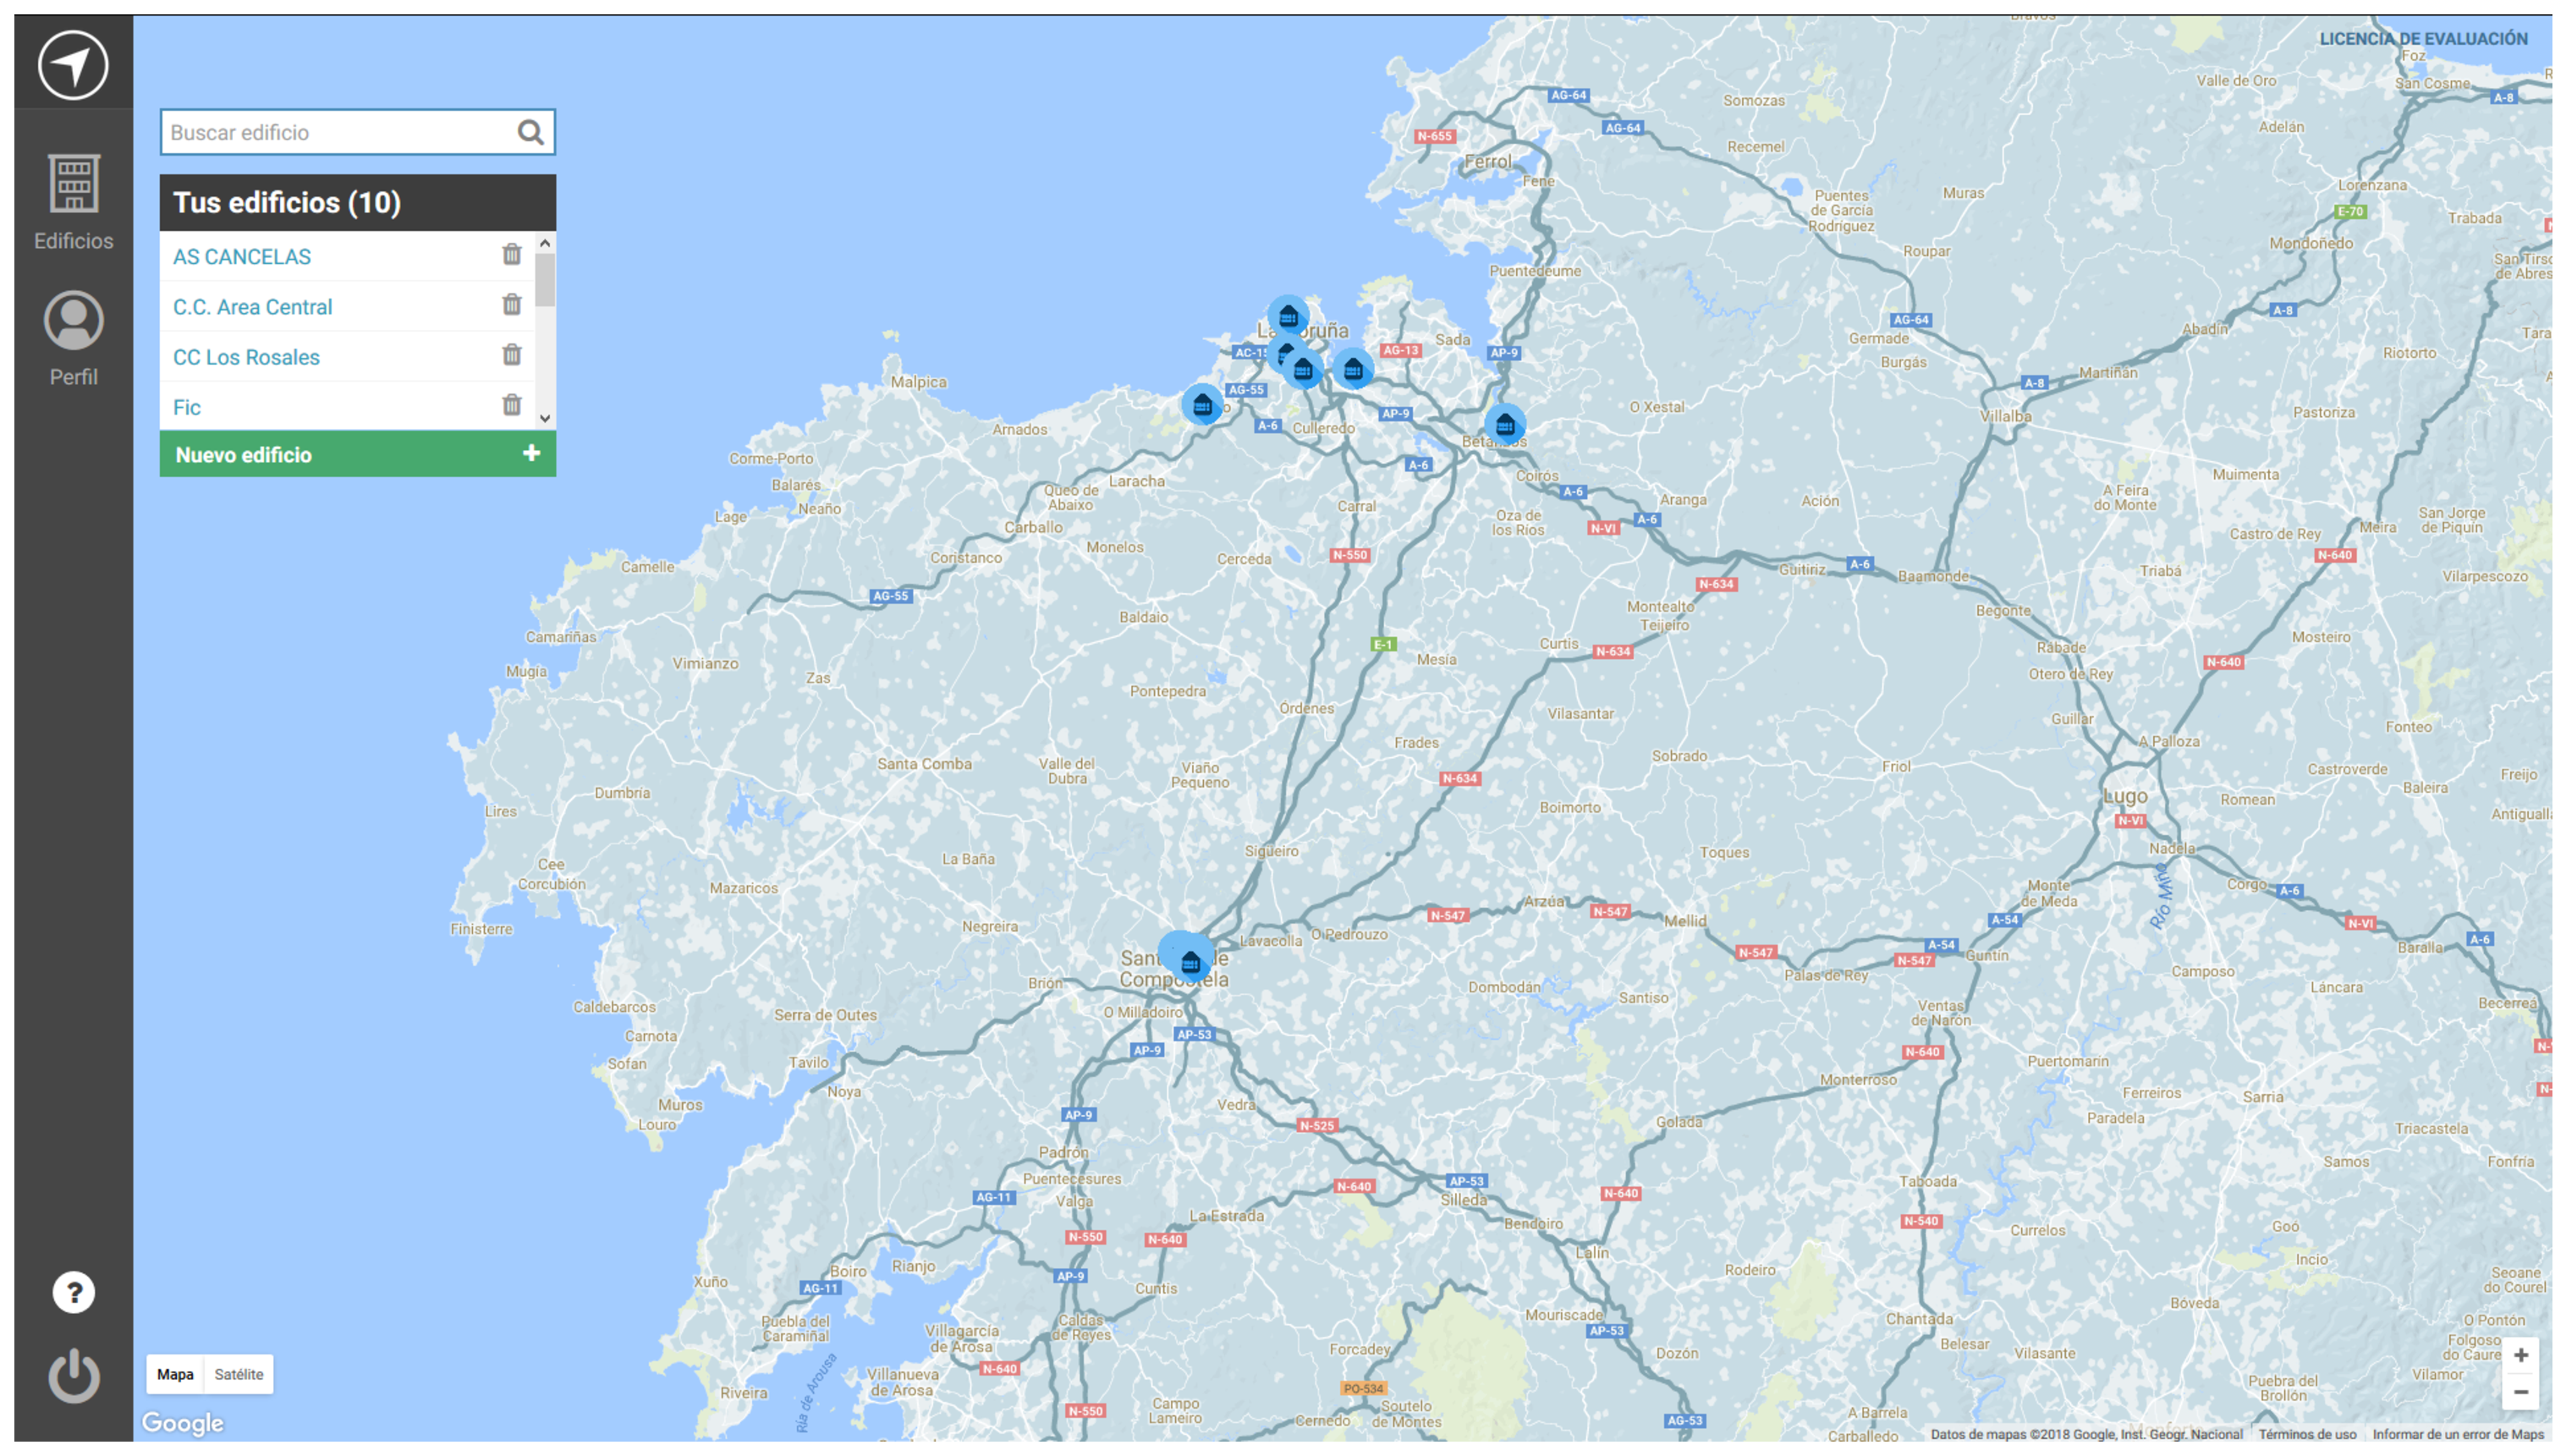
\includegraphics[width=0.65\textwidth]{figures/Capturas/dashboard}
		\caption{Vista inicial do dashboard de Situm.}
		\label{fig:dashboard}
	\end{center}
\end{figure}

\section{Editar edificios en Situm}
O dashboard de Situm permítenos a creación e edición de edificios. Ao abrilo veremos un mapa onde visualizaremos as posicións dos nosos edificios e unha lista á esquerda cunha relación dos mesmos. Dende aquí poderemos modificar os edificios xa existentes ou crear outros novos.
Para a creación dun novo edificio deberemos indicar a información do mesmo, coma o seu nome e unha descrición. No segundo paso debemos crear as súas plantas, para o cal precisaremos os seus planos. Para cada unha das plantas debemos situar o seu plano no mapa para que coincida co seu emprazamento real, podendo modificar a súa escala e rotalo. Este paso é básico para que funcione correctamente a localización no interior do edificio, polo que se debe axustar ao máximo os planos.
Na figura~\ref{fig:edificio} pódese observar a vista de modificación dun edificio.

\begin{figure}[tbh] 
	\begin{center}
		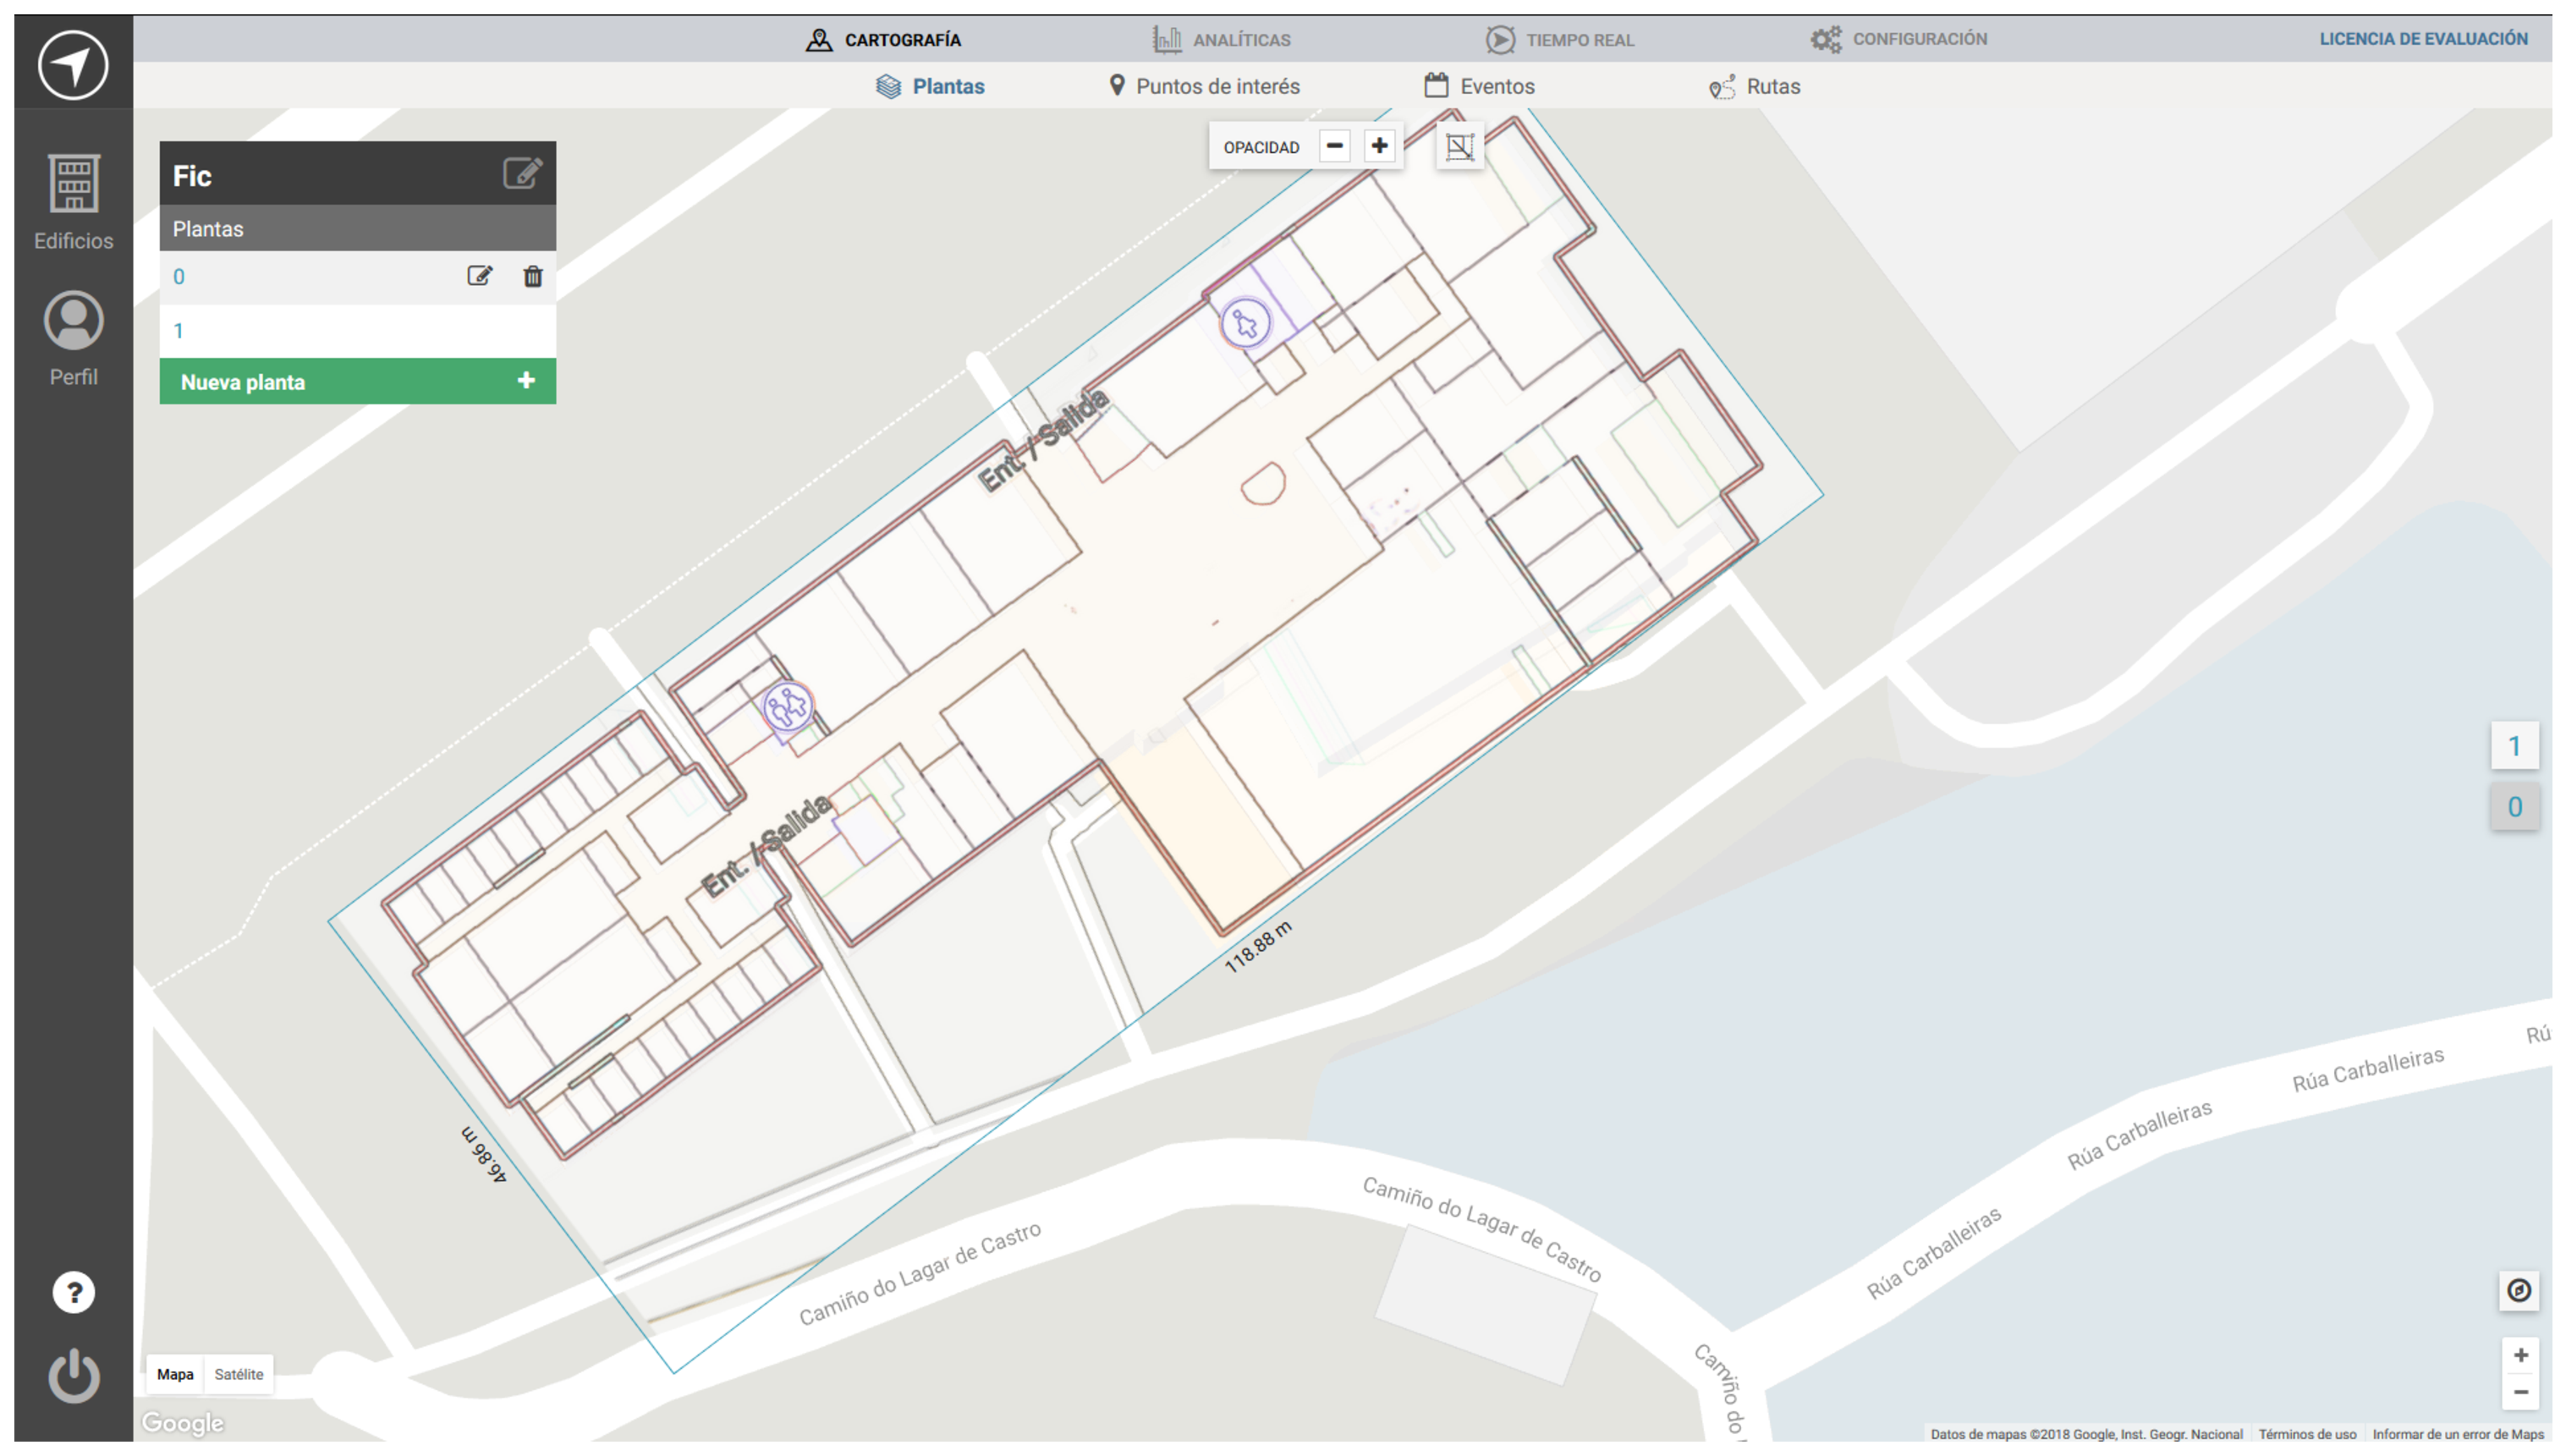
\includegraphics[width=0.65\textwidth]{figures/Capturas/edificio}
		\caption{Vista de modificación dun edificio.}
		\label{fig:edificio}
	\end{center}
\end{figure}

\section{Calibración de cada planta}
Para a calibración das plantas dos nosos edificios precisamos a aplicación de calibrado proporcionada por Situm: Situm Mapping Tool (ver figura~\ref{fig:mapping_tool}). É unha aplicación moi simple na que debemos indicar a nosa situación no mapa mentres nos movemos polo edificio. O obxectivo é cubrir a superficie de todas as plantas por onde poden pasar os usuarios.
O proceso de configuración é o seguinte: partindo dunha posición inicial, debemos indicar na aplicación a nosa situación. Posteriormente haberá que camiñar en liña o máis recta posíbel mentres indicamos cada poucos metros onde nos atopamos. Cando desexemos rematar con esa calibración temos que parala e enviala aos servidores de Situm. Haberá que repetir este proceso varias veces ata cubrir a superficie do edificio.
É recomendábel facer recalibracións periódicas dos edificios para non perder precisión.

\begin{figure}[tbh] 
	\begin{center}
		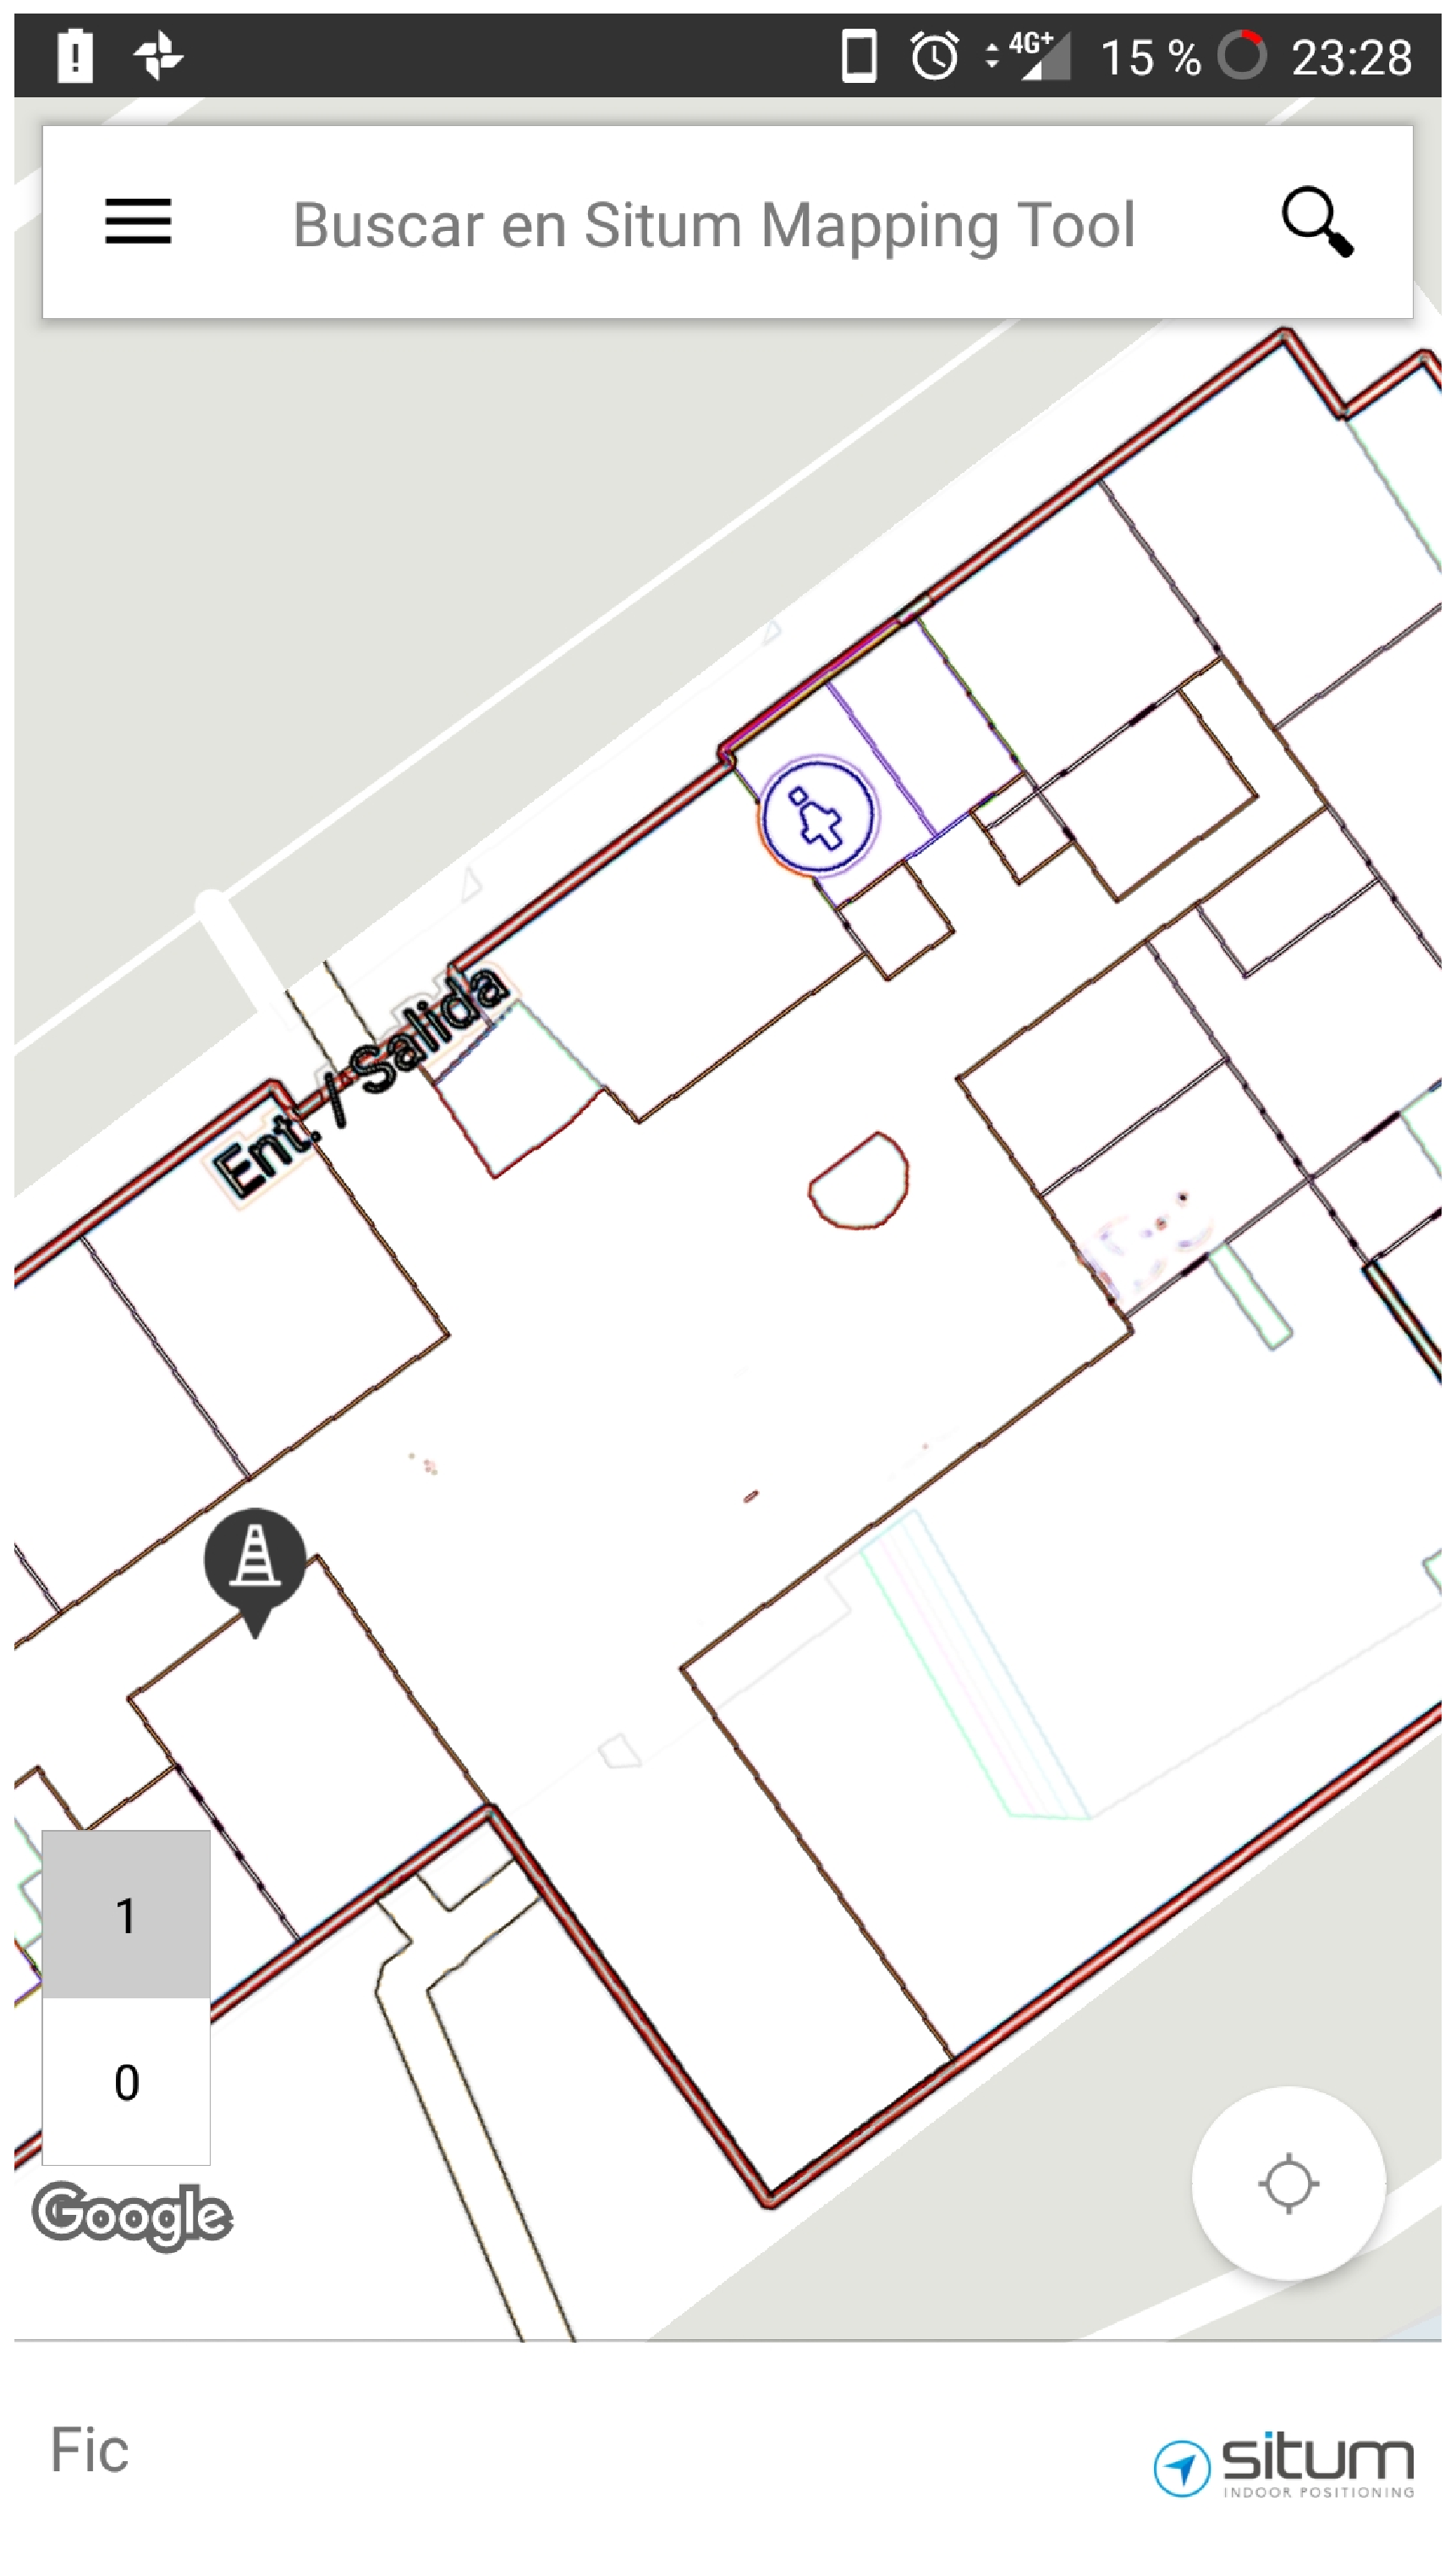
\includegraphics[width=0.65\textwidth]{figures/Capturas/mapping_tool}
		\caption{Aplicación de calibración: Situm Mapping Tool.}
		\label{fig:mapping_tool}
	\end{center}
\end{figure}

\section{Punto de interese Situm}
Situm dá a posibilidade da creación de puntos de interese propios para a realización de accións concretas. No noso sistema non facemos uso deles pois temos os nosos propios puntos de interese pero explícase o proceso de creación pois é unha das opcións máis útiles do seu sistema.
Dentro do dashboard de Situm e despois de seleccionar o edificio no que queremos crear os puntos de interese, escolleremos a pestana chamada "Puntos de interese". Chegado a este punto visualizaranse os mapas do edificio xunto cos puntos de interese xa creados, dispoñíbeis para a súa edición ou eliminación. Por suposto, tamén está dispoñíbel a creación de novos puntos, que poderemos situar directamente sobre o mapa e para os cales se dará algún tipo de información. Este proceso pode observarse na captura~\ref{fig:poi}

\begin{figure}[tbh] 
	\begin{center}
		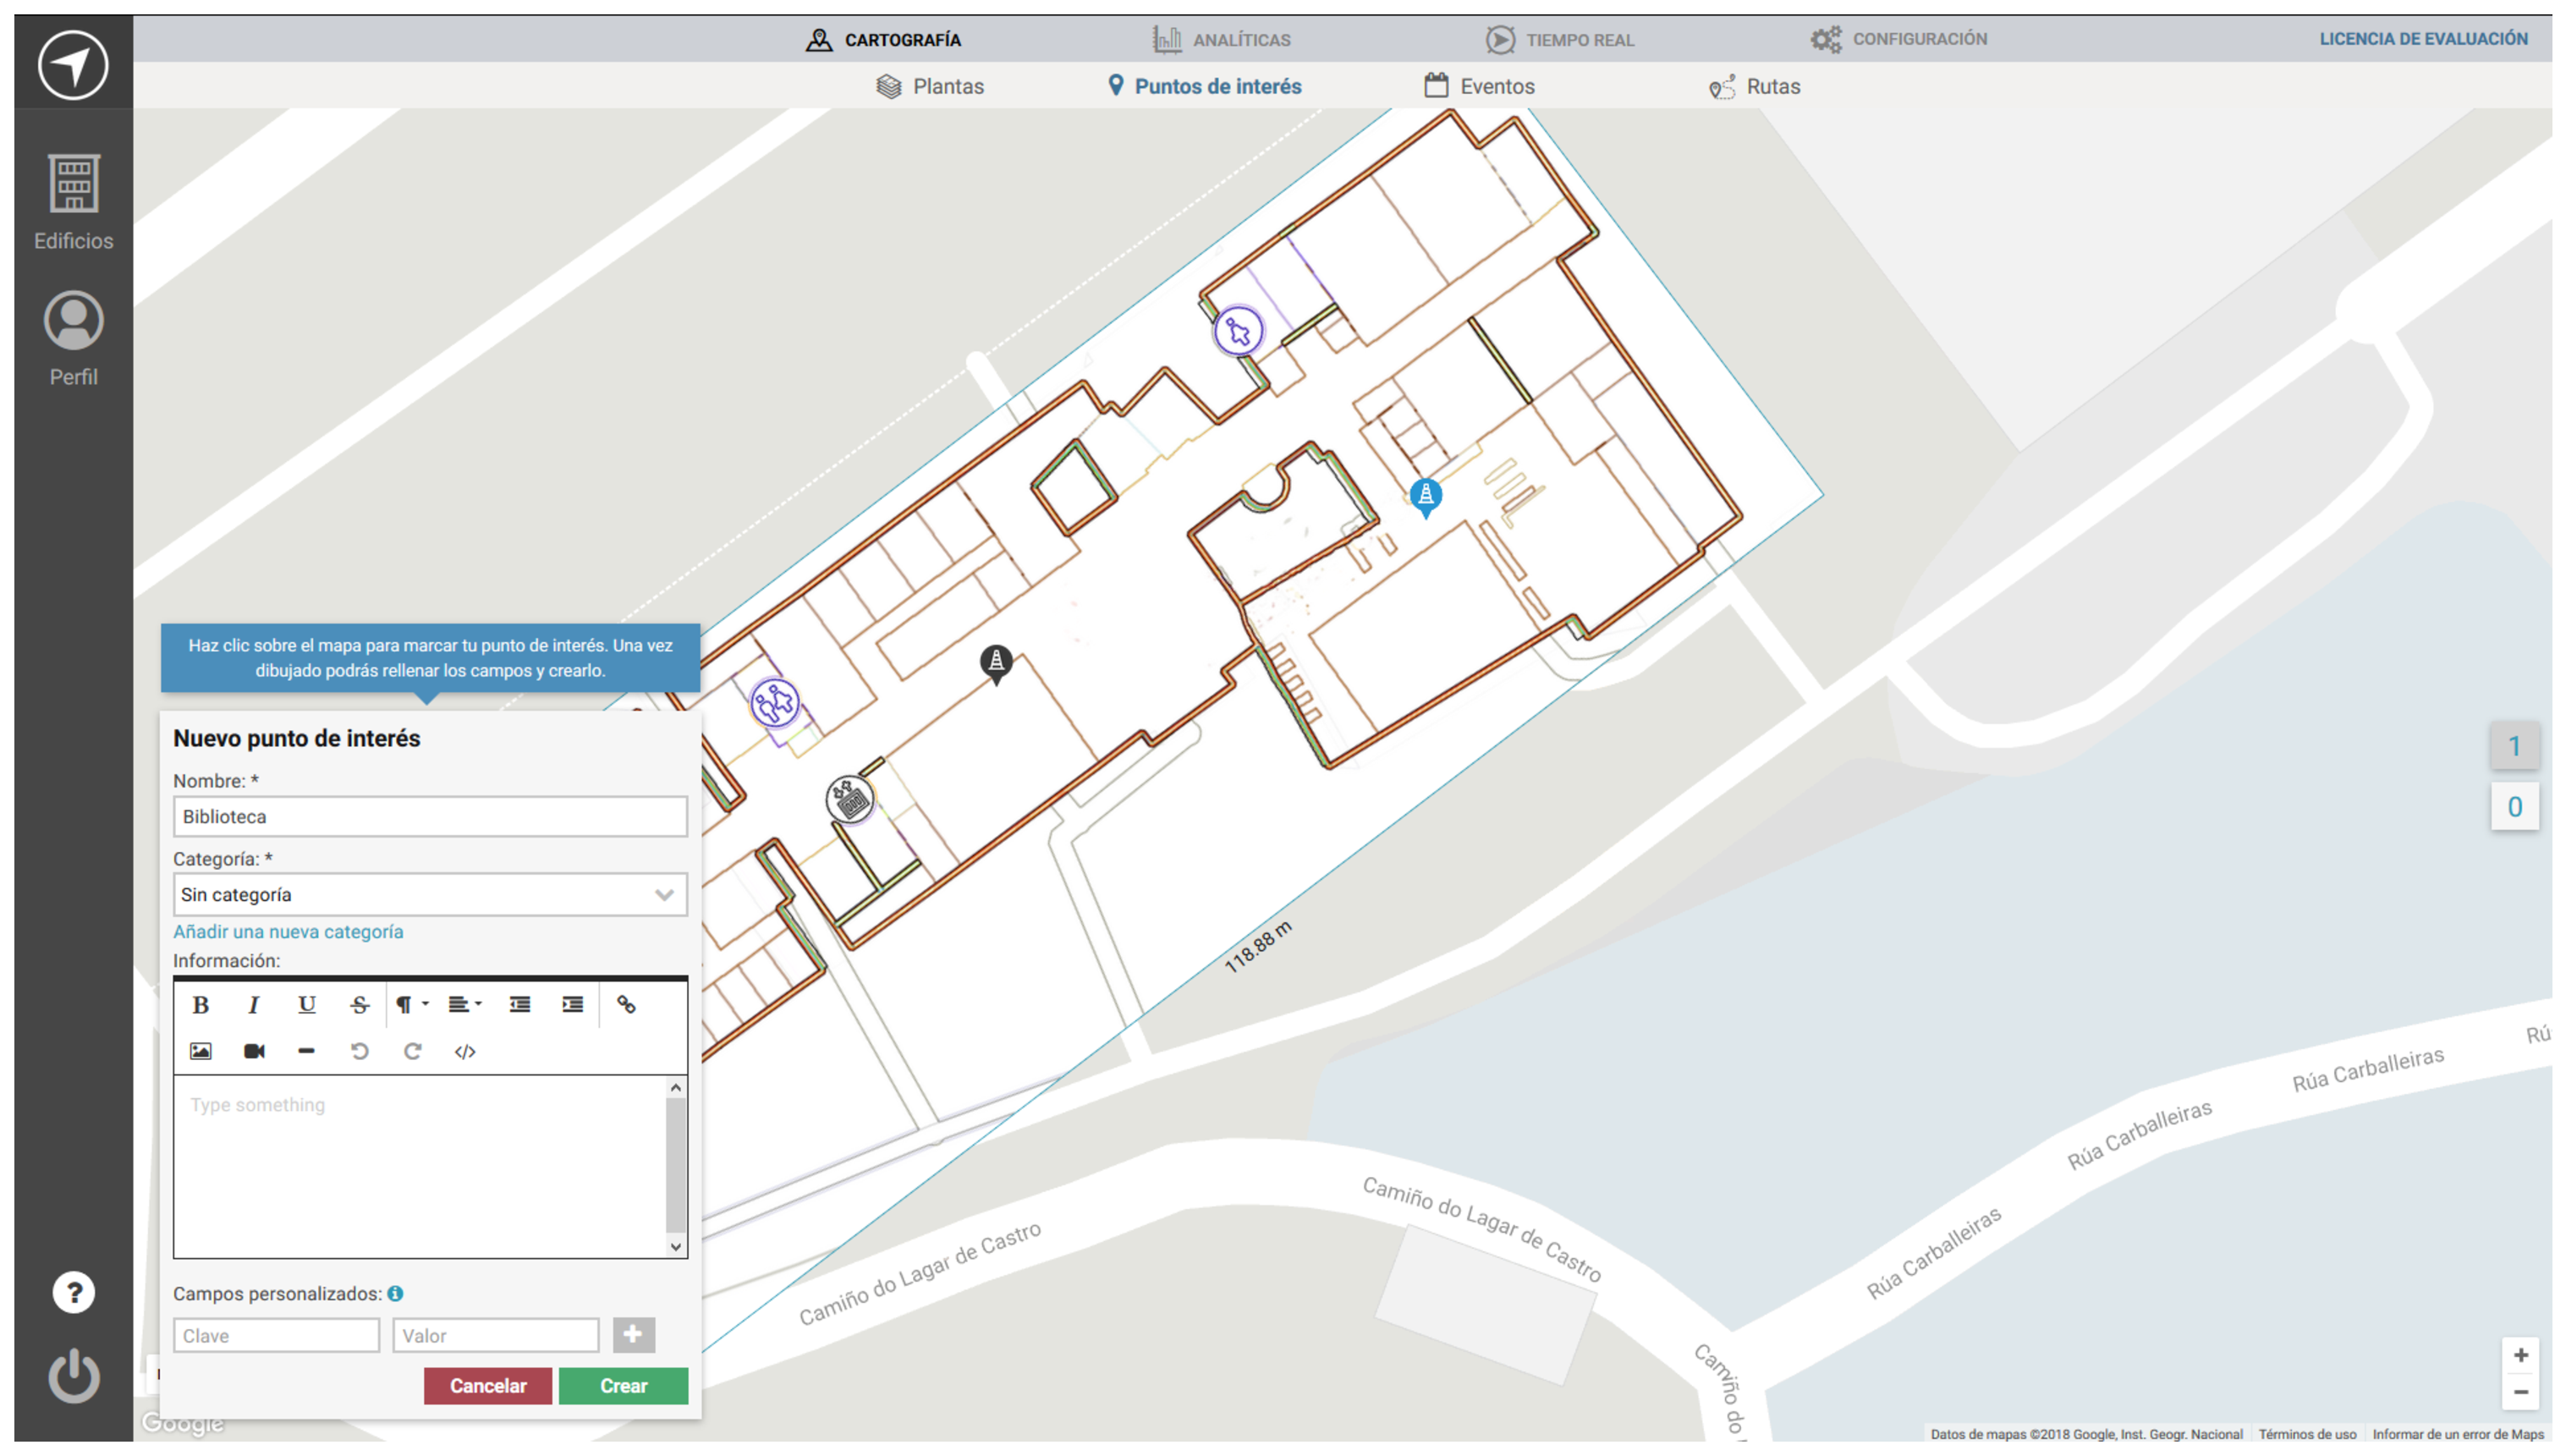
\includegraphics[width=0.65\textwidth]{figures/Capturas/poi}
		\caption{Proceso de creación de POIs en Situm.}
		\label{fig:poi}
	\end{center}
\end{figure}

\section{Definición de rutas}
No Dashboard hai unha sección dende a cal poderemos definir as rutas dentro do edificio. Dende ela pódense unir os distintos grafos creados por Situm na calibración do edificio para indicar as posíbeis rutas que poderán seguir os usuarios. Non hai máis que pulsar os grafos que queremos combinar para crear unha ruta. Tamén se permite a unión de puntos entre pisos distintos, facendo click sobre un dos puntos que se desexa unir para despois seleccionar o outro punto e marcar a opción. A captura~\ref{fig:rutas} mostra a ventá de definición de rutas.

\begin{figure}[tbh] 
	\begin{center}
		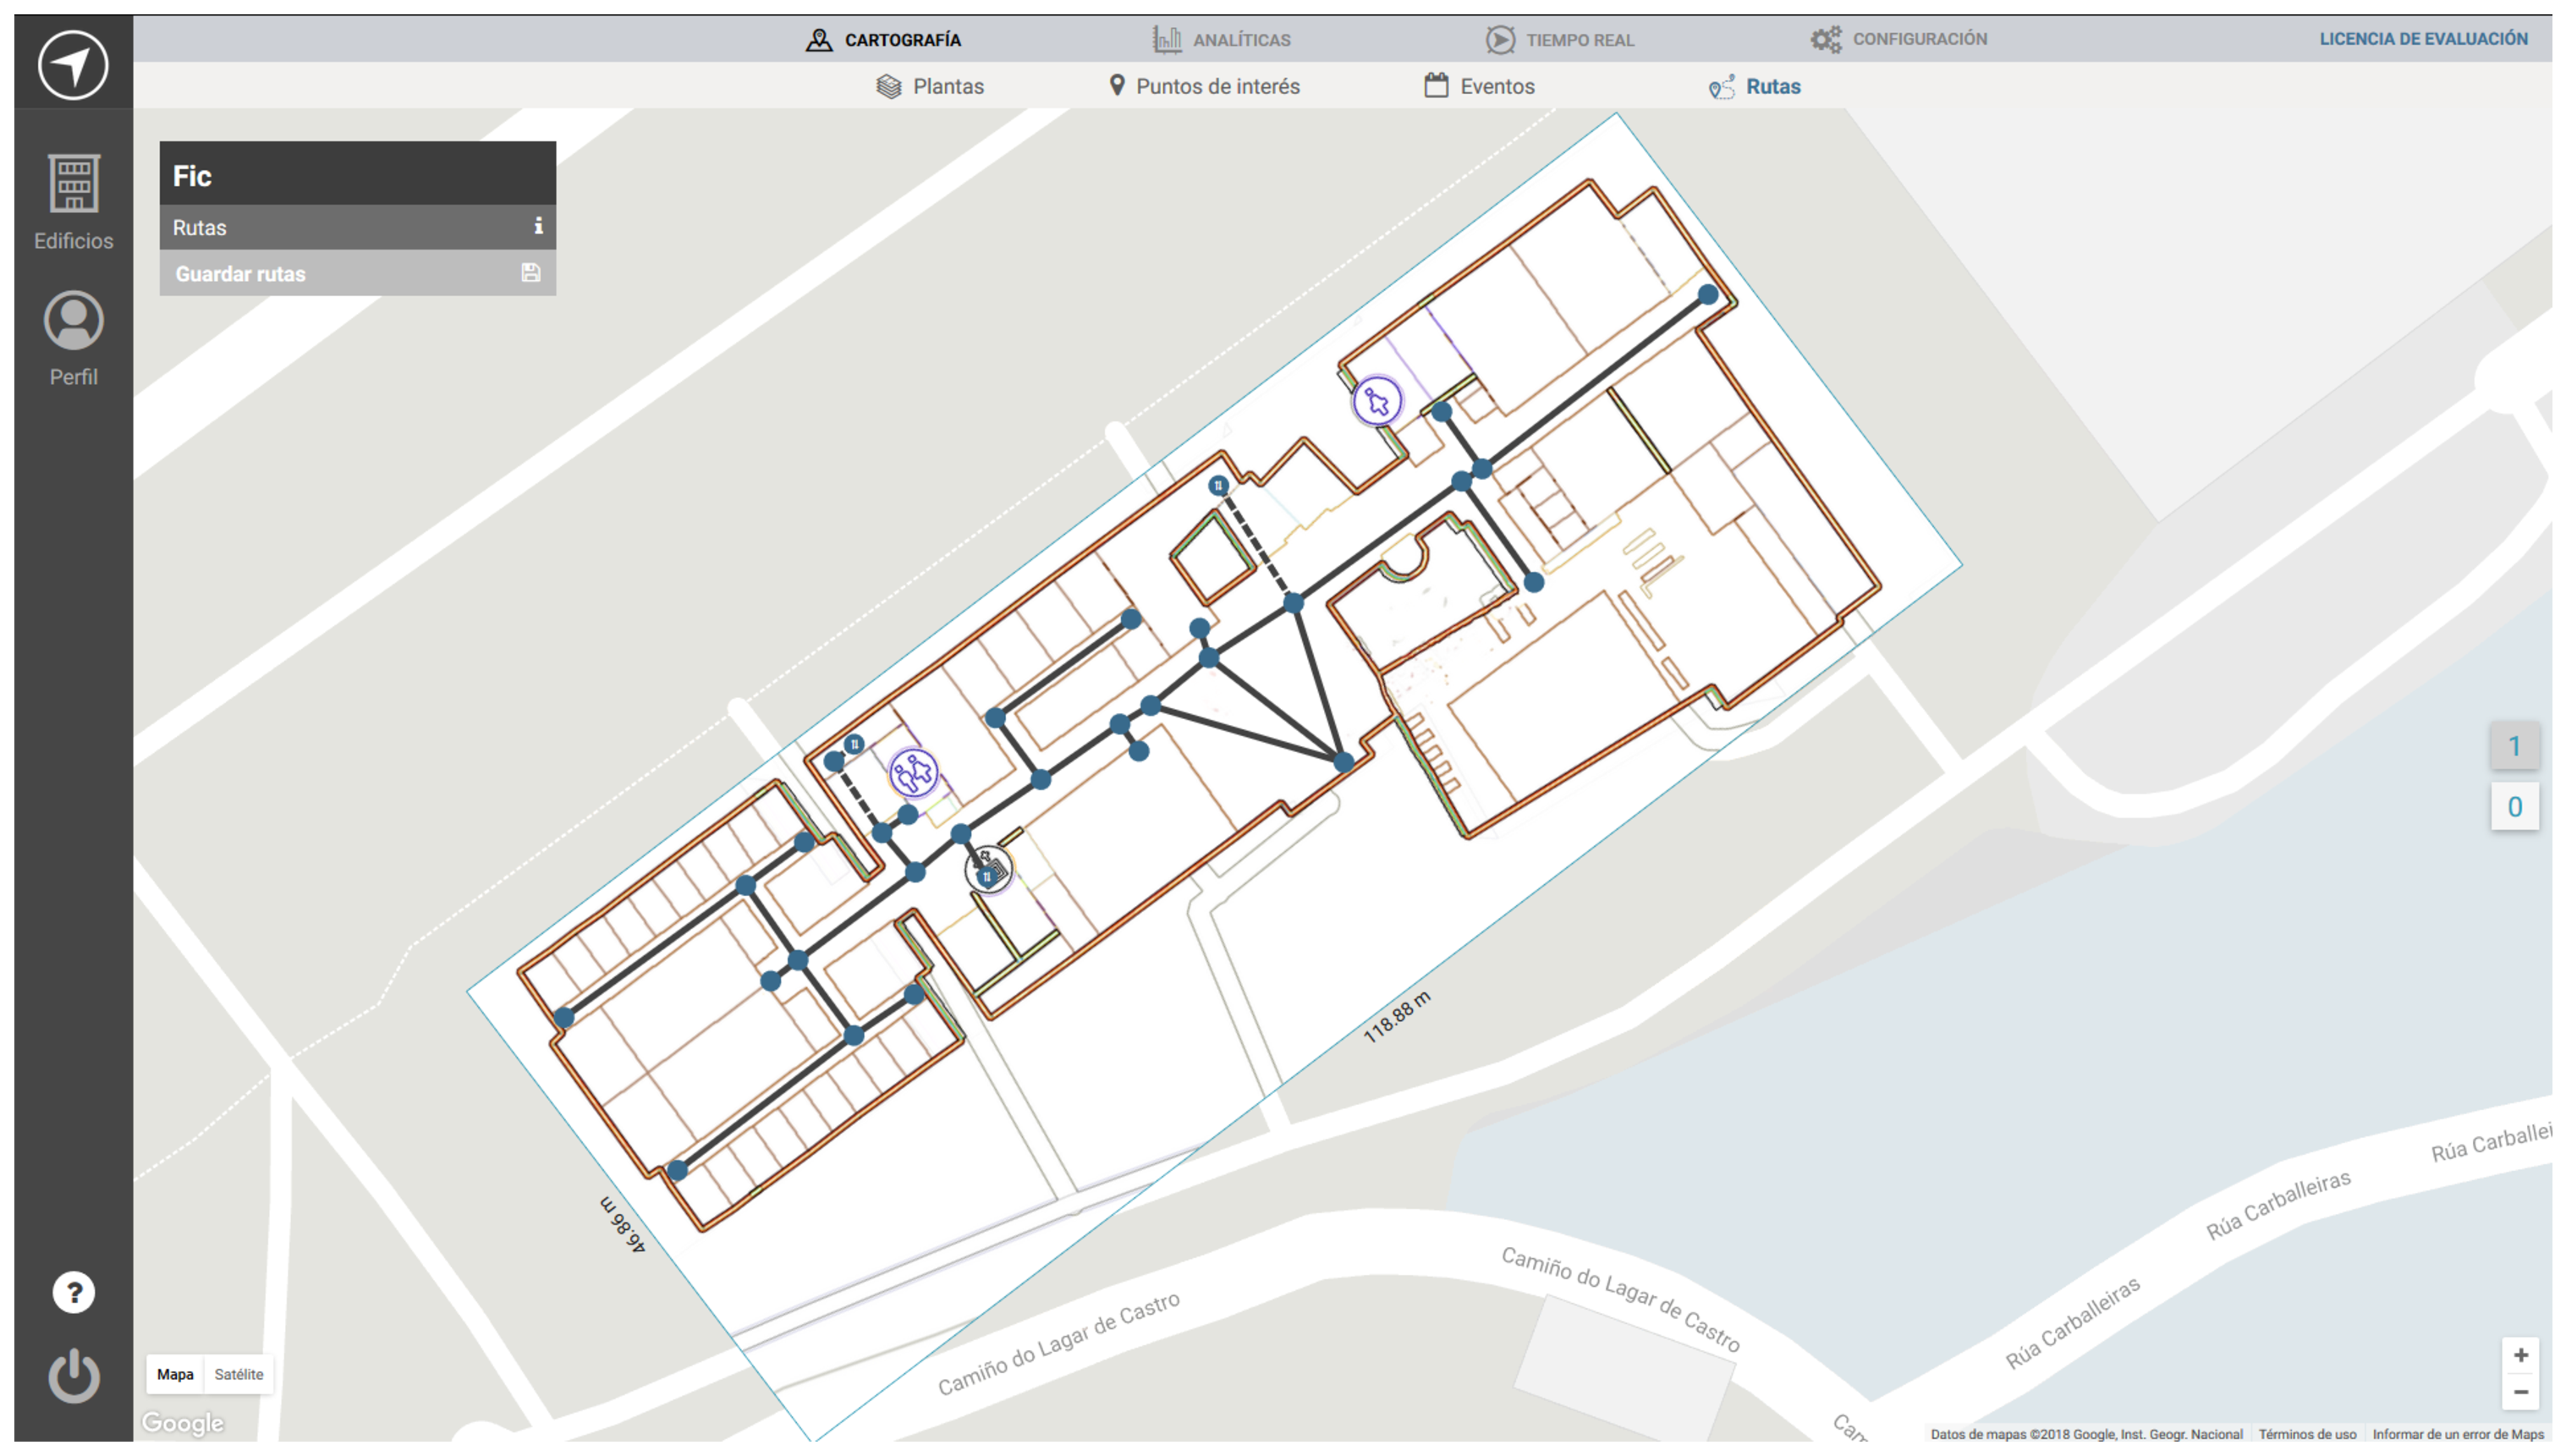
\includegraphics[width=0.65\textwidth]{figures/Capturas/rutas}
		\caption{Proceso de creación de rutas.}
		\label{fig:rutas}
	\end{center}
\end{figure}